\section{Type Ia Supernovae as Standard Candles}

Supernovae (SNe) are the explosion of stars at the end of their lives
that can be as bright as ten billion Suns for a period of a few
weeks. They are divided into subtypes empirically, based on the
properties of their optical spectra. The first division, into Types I
and II, was firmly established by \citet{minkowski41a}. Supernovae
whose spectra clearly exhibit hydrogen are Type II; those that do not
are Type I. These two main classes have since been
subdivided. Specifically for Type I, it was recognized that there are
spectroscopically distinguishable subsets in the mid-1980s
\citep{elias85a,panagia85a,wheeler85a,uomoto85a}. Type I SNe are now
divided into Ia, Ib and Ic. Type Ia SNe (SNe~Ia) are defined by the
presence of a strong Si II $\lambda6355$ absorption trough blueshifted
to $\sim 6100$\AA\ while Types Ib and Ic do not have this feature and
are divided by the presence (Ib) or absence (Ic) of clear helium I
lines \citep[see][for a review]{filippenko97a}.

Since the original division into Types I and II a more physical
dichotomy has become apparent: SNe~Ia are now widely accepted to be
thermonuclear disruptions of mass-accreting carbon-oxygen (C-O) white
dwarfs (WDs), while all other types are thought to result from the core
collapse of massive stars ($>8M_\odot$) at the end of their lives.
For SNe~Ia, the explosion is believed to occur as the white dwarf
nears the \citet{chandrasekhar31a} mass limit. That all SNe Ia occur at
nearly the same mass gives a natural explanation for the overwhelming
homogeneity exhibited by this (but not any other) type.

This homogeneity is what makes SNe~Ia the best available ``standard
candles'' that are visible at cosmological distances. Their peak
absolute $B$-band magnitudes have a dispersion of $\sigma(M_B) \sim
0.3$ \citep[e.g.,][]{hamuy96a}, excluding spectroscopically peculiar
SNe~Ia. Empirical correlations between absolute magnitude and other SN
properties can be used to effectively decrease this dispersion,
increasing their utility for cosmological measurements. The first and
most widely used such correlation is between the absolute
magnitude and the width of the SN light curve (or rate of decline):
brighter SNe have light curves that are wider, or
slower evolving. Characterizing the light curve width with the $\Delta
m_{15}$ \citep{phillips93a} or ``stretch''
\citep[$s$;][]{perlmutter97a} parameter, the dispersion of
``corrected'' peak magnitudes can be reduced to $\sigma(M_B^{\rm corr})
\sim 0.17$.

Today there are various methods used to parameterize SN~Ia light
curves and determine corrected magnitudes
\citep[e.g.,][]{guy05a,guy07a,jha07a,conley08a}. In addition to light
curve shape, a second parameter corresponding to the SN color is
used. For example, the {\sc salt} light curve fitter \citep{guy05a}
defines the corrected magnitudes as
\begin{equation}
M_B^{\rm corr} = M_B + \alpha (s-1) -\beta c
\end{equation}
where $c$ is the SN color, approximately equivalent to $E(B-V)$. With two
parameters the dispersion can be reduced to $\lesssim 0.15$~mag and
there is evidence that it can be reduced to $0.13$~mag or lower with
other correlations, such as with spectral line ratios \citep{bailey09a}.

In contrast to the handful of SNe~Ia used in the discovery of dark
energy over a decade ago \citep{perlmutter97a,riess98a,perlmutter99a},
over 500 SNe~Ia are now used in the latest analyses
\citep[e.g.][]{hicken09a,amanullah10a}, with at least as many more
observed and still ``in the pipeline.'' Combined with constraints from
baryon acoustic oscillations and the cosmic microwave background,
SNe~Ia constrain $\Omega_M = 0.277 \pm 0.014$ (stat)
$^{+0.017}_{-0.016}$ (stat+sys) and $w = -1.009
^{+0.050}_{-0.054}$(stat) $^{+0.077}_{-0.082}$ (stat+sys), assuming a
flat universe \citep{amanullah10a}.


\section{The Progenitors of SNe Ia}

Despite their very successful use as standard candles and the vast
numbers of them now observed, \emph{significant} uncertainties remain
about many aspects of SNe~Ia.  As noted above, we are quite certain
about the basic model of SNe~Ia: they are the thermonuclear explosion
of mass-accreting C-O WDs, and that furthermore the accreted mass is
donated by a binary companion star.  However, the nature of the
companion star, how the system evolves to trigger a SN~Ia, and how the
explosion starts and progresses are still unknown 
\citep[see][for a review]{livio01a}.

The nature of the companion and the evolution of the system prior to
explosion are collectively referred to as the progenitor scenario. In
addition to the intrinsic interest in the SNe themselves, a better
understanding of the progenitor scenario is demanded from both a
cosmological and an astrophysical perspective.
Cosmologically, the corrections that improve the standardization of
SNe~Ia are entirely based on \emph{empirical} relations, and not a
deep understanding of the events themselves.  While the unknown nature
of the SN progenitor system is unlikely to bias measurements at the
current level of uncertainty \citep{yungelson00a,sarkar08a}, it could
become a significant source of uncertainty in the future as
statistical uncertainty continues to decrease. Essentially, it leaves
open the question of whether high-redshift SNe are different than
low-redshift SNe in a way that affects the inferred distance.
Astrophysically, SNe~Ia dominate the production of iron
\citep[e.g.,][]{matteucci86a,tsujimoto95a,thielemann96a} and provide
energy feedback \citep{scannapieco06a} in galaxies. To properly
include these effects in galaxy evolution models requires an accurate
prediction of the SN~Ia rate in galaxies of varying ages, masses and
star formation histories, which in turn requires a good understanding
of the progenitor. This is particularly true for higher redshifts
where direct SN rate constraints are unavailable.


\subsection{Models}

The leading models fall into two classes: the {\it single degenerate}
scenario \citep[SD;][]{whelan73a,nomoto82a}, and the {\it double
  degenerate} scenario \citep[DD;][]{iben84a,webbink84a}. In the SD
scenario the companion is a red giant or main sequence star that
overflows its Roche lobe. In the DD scenario, the companion is a
second C-O WD which merges with the primary after orbital decay due to
the emission of gravitational radiation.  Within the SD class of
models there are various refinements: The companion could be a red
giant donating hydrogen or a subgiant donating helium rich material,
or even a main sequence star in close orbit. The explosion could occur
very near the Chandrasekhar mass or significantly below it.
Among DD models there is less room for refinement as both stars are
necessarily WDs. However, their total mass and their mass ratios are
open questions. For example, \citet{vankerkwijk10a} have recently
suggested sub-Chandrasekhar mass systems with WDs of roughly equal
mass as a promising progenitor candidate.

It is possible to probe the progenitor scenario via direct
observations, such as imaging of SN
remnants \citep[e.g.,][]{ruizlapuente04a,ihara07a,maoz08a,gonzalez09a},
the observation of hydrogen in SN spectra \citep[e.g.,][]{livio03a},
X-ray detection before
explosion \citep[e.g.,][]{nelemans08a,roelofs08a,gilfanov10a}, or
searches for likely progenitor
systems \citep[e.g.,][]{geier07a,parthasarathy07a}. Drawing definitive
conclusions based on such observations is typically quite difficult,
due in part to the rarity of very nearby SNe~Ia, and in part to the
fact that even the direct detection of one type of progenitor scenario
cannot rule out a contribution from the other scenario.

Along these lines, note that recently the observation of SNe~Ia with
super-Chandrasekhar mass progenitors \citep{howell06a,scalzo10a} has
been taken as evidence in favor of the DD scenario. However, there is
some confusion about how this can be achieved in the DD scenario, as
the lighter WD is expected to dissipate into a disk in the merger
process. Even if these SNe are found to originate from DD progenitors,
they represent only a small subset of all SNe~Ia; the bulk of SNe may
be explained by a different mechanism.

\section{SN~Ia Rates and the Delay Time Distribution}

An alternative to direct detection is to probe the progenitor scenario
statistically by measuring the rate at which SNe~Ia occur
\citep[e.g.,][]{ruizlapuente95a,ruizlapuente98a,yungelson00a}.  SN~Ia
rates constrain the progenitor scenario via the delay time
distribution (DTD), $\Psi (t)$, where ``delay time'' refers to the time between
star formation and SN~Ia explosion. The DTD is the distribution of
these times for a population of stars, and is equivalent to the SN~Ia
rate as a function of time after a burst of star formation. Crucially,
the delay time is governed by different physical mechanisms in the
different progenitor scenarios. For example, in the DD scenario,
the delay time is dominated by the time the orbit takes to decay due to
gravitational radiation. In the SD scenario, when
the donor is a red giant star the delay time is set by the time the
companion takes to evolve off the main sequence. 

To see how these dependencies translate to different DTDs for a
population of stars, we consider a simplified model for each
scenario. For the DD scenario, we make the approximation that the time
to form a double WD binary is negligible compared to the gravitational
radiation merger time. That time depends on the the initial WD
separation ($a$) as
\begin{equation}
t \propto a^4.
\end{equation}
Assuming the initial separations are distributed as a power law,
\begin{equation}
\frac{dN}{da} \propto a^\epsilon ,
\end{equation}
the SN rate as a function of time (DTD) is given by 
\begin{equation}
\Psi (t) = \frac{dN}{dt} = \frac{dN}{da} \frac{da}{dt} \propto 
t^{(\epsilon -3)/4} \quad {\rm (DD~scenario).} 
\end{equation}
For the SD scenario with a red giant companion star, we similarly
neglect the time to form the WD and assume that the delay time is
equal to the main-sequence lifetime of the secondary (lower mass)
star. If that lifetime depends on the mass as a power law,
\begin{equation}
t \propto m^\delta,
\end{equation}
and if we assume the initial mass function (IMF) follows a power law as well,
\begin{equation}
\frac{dN}{dm} \propto m^\lambda ,
\end{equation}
then the DTD is given by
\begin{equation}
\Psi (t) = \frac{dN}{dm} \frac{dm}{dt} \propto t^{(1+\lambda-\delta)/\delta}
\quad {\rm (SD~scenario)}.
\end{equation}
Plugging in nominal values of $\epsilon = -1$ for the DD scenario (the
approximate separation distribution observed in binary systems) and the
commonly used value $\delta = -2.5$ and the \citet{salpeter55a} slope
$\lambda=-2.35$ for the SD scenario, we arrive at $\Psi (t) \propto
t^{-1}$ for the DD scenario and $\Psi (t) \propto t^{-0.46}$ for the
SD scenario.

These models serve to illustrate how the shape of the DTD can be
affected by the progenitor, but in both cases these are
oversimplifications. In the DD model, although the distribution of
initial binary separations is observed to be approximately $\propto
a^{-1}$, the distribution of separations after the system has passed
through two common envelope \citep[CE; see, e.g.,][]{yungelson05a}
phases is not known. It is could be radically different, resulting in
a power law much different than  $\Psi (t) \propto t^{-1}$. Furthermore, at small delay
times, the DTD will not follow a power law at all, as WDs do not form
instantaneously, but take from 40 -- 400 Myr after star formation.  In
the SD scenario, the slope of the DTD can actually be much steeper
than $\sim$$t^{-0.5}$ at later times. This is because in an older
population, fewer and fewer secondary stars will have the required
envelope mass to to donate to the primary so that it can reach $1.4
M_\odot$. In addition, factors such as the IMF, the distribution of
initial separation and mass ratio in binary systems, are not perfectly
known and will affect the derived DTD.

Detailed delay time distributions attempting to take these and other
effects into account were computed analytically following the proposal
of both the SD \citep{greggio83a} and DD
\citep{tornambe86a,tornambe89a} scenarios. Later, theoretical DTDs
were extended to include various subclasses of each model and a wider
range of parameters \citep{tutukov94a,
  yungelson00a,matteucci01a,belczynski05a,greggio05a}. More recently,
binary population synthesis codes have been used to compute the DTD
numerically, following a population of binaries with chosen initial
conditions through the stages of stellar and binary evolution. In
recent such studies, different plausible prescriptions for the initial
conditions and for the binary evolution have lead to widely ranging
DTDs, even within one scenario
\citep{hachisu08a,kobayashi09a,ruiter09a,mennekens10a}. Figure~\ref{fig:dtd_mennekens10a}
shows an example of various DTDs from \citet{mennekens10a}. A
measurement of the DTD then must constrain not only the relative
contribution of various progenitor scenarios, but also the initial
conditions and CE phase, which is particularly poorly
constrained. Still, most simulations show a difference in the DTD
shape between the SD and DD scenarios: the SD scenario typically shows
a strong drop-off in the SN rate at large delay times, whereas this is
not seen in the DD scenario \citep[but see][]{hachisu08a}.

\begin{figure}[tbh]
\begin{center}
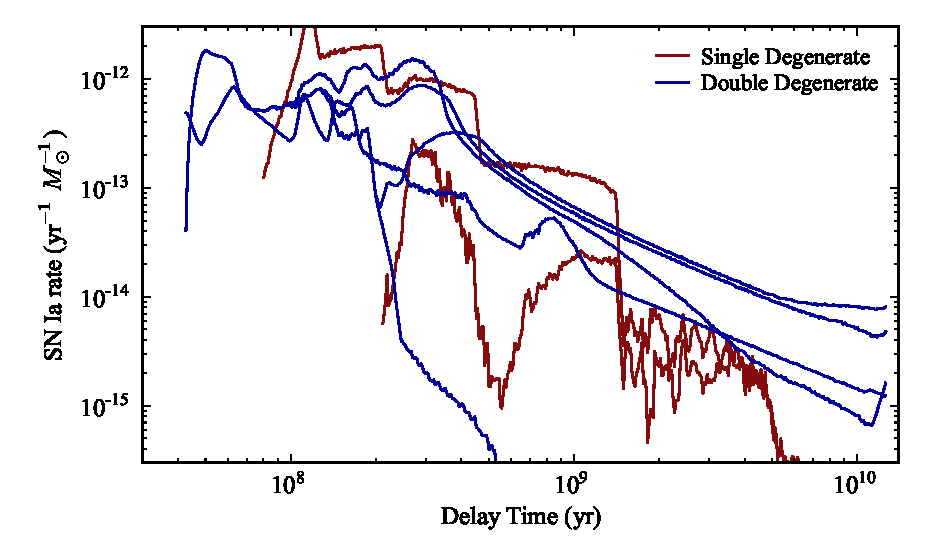
\includegraphics[width=\textwidth]{figures/review/dtd_mennekens10a.eps}
\end{center}
\caption[Example of delay time distributions]{An example of delay time
  distributions calculated using stellar population synthesis models
  from \citet{mennekens10a}. The various single degenerate and double
  degenerate DTDs use different assumptions and prescriptions for
  common envelope evolution.\label{fig:dtd_mennekens10a}}
\end{figure}

\section{Constraints from SN~Ia Rates}

As the DTD is simply the SN~Ia rate as a function of time after star
formation, it can be measured empirically by measuring the SN rate in
stellar populations of many different ages. In practice, this is
difficult because the typical galaxy is made up of many stars of
different ages. When a SN~Ia explodes, it is usually impossible to
tell which particular population the SN came from.

Five years ago, we had very little information about the shape of the
DTD from an observational standpoint. It had been recognized much
earlier that the SN~Ia rate is higher in star-forming galaxies
\citep{vandenbergh90a}, implying that the DTD is largest at small
delay times. [In fact, even earlier this trend was suggested as a
  motivation for two distinct subsets of SNe~I by
  \citet{dallaporta73a}.] However, little detail was gained over the
next 15 years. Some recent measurements have confirmed the same trend
with larger samples \citep{mannucci05a}. This has lead to a
parameterization of the DTD with a ``two component'' model
\citep{scannapieco05a} in which one component is proportional to the
instantaneous star formation rate and the other component is
proportional to stellar mass:
\begin{equation}
\mathcal{R}_{\rm SN~Ia} (t) = A M_\star (t) + B \dot{M}_\star(t).
\end{equation}
Also known as the ``$A+B$'' model, this form is convenient for
predicting the SN rate in environments with varying amounts of recent
star formation, and its parameters can be measured with relative ease
\citep[e.g.,][]{sullivan06a}. However, it suffers from being
unphysical (the $B$ component implies a delay time of zero) and
lacking theoretical motivation.  Unfortunately, this simplified model
was often interpreted as evidence for two distinct populations of
progenitors \citep[e.g.,][]{mannucci06a}, even though a single
progenitor channel could easily reproduce the observed
data. Complicating the entire situation at the time, some measurements
produced results in contradiction with the existence of short
delay-time SNe~Ia.  For example, \citet{dahlen04a} found the
volumetric SN~Ia rate (discussed in greater detail below) to decrease
at $z \gtrsim 1$, implying a narrow DTD centered at $t \sim 3$~Gyr,
with no contribution from short-delay SNe \citep{strolger04a}.

Recently, more detailed measurements of the DTD have become possible
using a variety of methods. Several measurements have confirmed that
the delay time spans a wide range, from less than 100 Myr
\citep[e.g.,][]{aubourg08a} to many Gyr
\citep[e.g.,][]{schawinski09a}. Detailed spectroscopic host galaxy
information for a large SN sample has allowed better constraints on
stellar population ages \citep{brandt10a}. The DTD at intermediate
delay times has been accessed using early-type galaxies
\citep{totani08a}. The common wisdom arising from these measurements
is that the SN rate generally declines with time, and that SNe with
progenitor ages $\lesssim$ a few hundred Myr comprise perhaps
$\sim$50\% of all SNe~Ia. 

We now discuss two particular approaches to DTD measurements that are
the main subject of this thesis: volumetric rates and rates
specifically in galaxy clusters.


%This is consistent with volumetric SN~Ia rate measurements
%\citep[e.g.][]{neill06a,dilday10a,dahlen04a,poznanski07a,kuznetsova08a,
%dahlen08a}
%which show that the SN~Ia rate clearly increases with redshift over
%the range $0<z<1$.

%The SN rate may also depend on metallicity of the progenitors, so
%measurements in stellar populations of different metallicity may shed
%light too.

\subsection{The Volumetric Field Rate}

One particular method for measuring the DTD is to correlate the cosmic
star formation history (SFH) with the the cosmic SN~Ia rate as a
function of redshift \citep{yungelson00a}: the rate as a function of
cosmic time is simply the cosmic SFH convolved with the DTD. Knowing
the SFH to good accuracy and measuring the SN~Ia rate, one can work
out the DTD.

A decade ago, before this method had ever been implemented, it was not
always looked upon as having great promise. Mario Livio, for one, took
this view in his review of SN~Ia progenitors:
\begin{quote}
The progenitors can be identified from the observed frequency of SNe
Ia as a function of redshift, since different progenitor models
produce different redshift distributions. Personally, I think it would
be quite pathetic to have to resort to this possibility.
\begin{flushright}
-- Mario \citet{livio01a}
\end{flushright}
\end{quote}
However, in the intervening ten years, this method has gained
appeal. In part, this has been because direct detection methods (such
as spectroscopic detection of hydrogen in SNe~Ia) have still not
provided definitive answers as hoped. At the same time advances in SN
rate measurements and new methods for backing out the DTD have started
yielding constraints that are informing progenitor models
\citep[e.g.][]{vankerkwijk10a}.

A measurement of the volumetric SN~Ia rate is often a ``free''
byproduct of conducting a survey for SNe for cosmology
measurements. As a result, the rate has now been measured in many
different SN surveys at redshifts $0<z<1$
\citep[e.g.]{pain02a,neill07a}. For some time, a number of
measurements were in disagreement. However, with new precise results
at low redshift \citep{dilday10a,li10a} and the recently revised rates
from the IfA Deep survey \citep{rodney10a}, most measurements at $z<1$
have now come into agreement, and paint a consistent picture of a SN
rate increasing with redshift. These measurements are reaching the
precision necessary for a DTD measurement: the slope of the increase
at low redshift ($z \lesssim 0.3$) alone has recently been used to
constrain the DTD \citep{horiuchi10a}.  However, due to the difficulty
of detecting $z \gtrsim 1$ SNe from the ground, measurements at these
higher redshifts have been limited to SN searches in the
GOODS\footnote{Great Observatories Origins Deep Survey
  \citep{giavalisco04a}} fields
\citep{dahlen04a,kuznetsova08a,dahlen08a} using \emph{HST} and
ultra-deep single-epoch searches in the Subaru Deep Field (SDF) from
the ground \citep{poznanski07a,graur11a}. These studies have yielded
discrepant results for both the SN rate and the implications for the
DTD. The first $z>1$ measurements by \citet{dahlen04a} \citep[and
  later][with an expanded dataset]{dahlen08a} showed a rate that
peaked at $z \sim 1$ and decreased in the highest redshift bin at
$z>1.4$. However, an independent analysis of much of the same dataset
by \citet{kuznetsova08a} resulted in a substantially lower rate at $z
\sim 1$ and an inability to distinguish a falling rate at high
redshift. The recent results of \citet{graur11a} from the SDF also
show a substantially lower rate at $z \sim 1$, at the level of
$\sim$$2\sigma$ (statistical-only) in each of two bins compared to
\citet{dahlen04a}. Their results are consistent with a flat SN rate at
$z \gtrsim 1$, and were used to infer a DTD proportional to a power
law in time with index of approximately $-1$.

Relative to the \emph{HST} measurements, the SDF measurements have the
advantage of better statistics in the highest-redshift bin,
but \emph{HST} measurements hold advantages in systematics.  A rolling
search with \emph{HST} offers multiple observations of each SN and
much higher resolution than possible from the ground, useful for
resolving separation between SNe and their hosts. These factors lead
to a more robust identification of SNe~Ia relative to the SDF searches
where a single observation is used for both detection and photometric
typing. In addition, the \citet{dahlen08a} analysis used spectroscopic
typing in addition to photometric typing, whereas \citet{graur11a}
uses only photometric typing. In general, the very different
strategies employed make \emph{HST} measurements a good cross-check
for the SDF measurements and vice versa. Increasing the statistics
in \emph{HST} rate measurements can help in resolving the source of
the discrepancies between the two measurements. At the same time, it
is important to carefully consider the assumptions about SN properties
that have gone into each measurement. Illustrating this importance is
the significant difference between the results
of \citet{kuznetsova08a} and \citet{dahlen08a} despite a largely
overlapping dataset.

In chapter~\ref{sec:fieldrate} of this thesis, we address these issues
by (1) supplementing current determinations of the \emph{HST}-based $z
\gtrsim 1$ SN~Ia rate and (2) comparing the effect on results of
different dust distributions assumed in previous analyses.


\subsection{Cluster Rates}

As an alternative to volumetric SN~Ia rates where stellar populations
with a wide range of ages contribute at all redshifts, it is more
straightforward to extract the DTD in stellar populations with a
narrow range of ages (with a single burst of star formation being the
ideal). Galaxy clusters, which are dominated by early-type galaxies,
provide an ideal environment for constraining the shape of the DTD at
large delay times. Early-type galaxies are generally expected to have
formed early ($z \gtrsim 2$) with little star formation since
\citep{stanford98a,vandokkum01a}. Cluster early-type galaxies in
particular form even earlier than those in the field, with most star
formation occurring at $z \gtrsim 3$
\citep{thomas05a,sanchezblazquez06a,gobat08a}.  Measuring the cluster
SN~Ia rate over a range of redshifts from $z=0$ to $z>1$ provides a
measurement of the SN~Ia rate at delay times from $\sim$2 to 11
Gyr. Obtaining an accurate rate at the highest-possible redshift is
crucial for constraining the shape of the late-time DTD: a larger
redshift range corresponds to a larger lever arm in delay time.

In addition to DTD constraints, there are also strong motivations for
measuring the cluster SN~Ia rate from a perspective of cluster
studies. SNe~Ia are an important source of iron in the intracluster
medium \citep[e.g.,][]{loewenstein06a}. Cluster SN rates constrain the
iron contribution from SNe and, paired with measured iron abundances,
can also constrain possible enrichment mechanisms \citep{maoz04a}. The
high-redshift cluster rate is particularly important: measurements
show that most of the intracluster iron was produced at high
redshift \citep{calura07a}. The poorly-constrained high-redshift
cluster rate is one of the largest sources of uncertainty in
constraining the metal-loss fraction from galaxies \citep{sivanandam09a}.

Cluster SNe~Ia can also be used to trace the
diffuse \emph{intracluster} stellar component. Intracluster stars,
bound to the cluster potential rather than individual galaxies, have
been found to account for anywhere from $5\%$ to $50\%$ of the stellar
mass in clusters \citep[e.g.,][]{ferguson98a,feldmeier98a,
gonzalez00a,feldmeier04a,lin04a,zibetti05a,gonzalez05a,krick06a,mihos05a}.
The use of SNe~Ia as tracers of this component was first demonstrated
by \citet{galyam03a} who found two likely host-less SNe~Ia out of a
total of seven cluster SNe~Ia in $0.06 < z < 0.19$ Abell
clusters. After correcting for the greater detection efficiency of host-less
SNe, they determined that on average, the intracluster medium
contained $20^{+20}_{-12}$\% of the total cluster stellar mass.  The
intrinsic faintness of the light from intracluster stars, combined
with $(1+z)^4$ surface brightness dimming, makes surface brightness
measurements impossible at redshifts much higher than $z=0.3$.  Type
Ia supernovae, which are detectable up to and beyond $z=1$, provide a
way to measure the intracluster stellar component and its possible
evolution with redshift.

The cluster SN~Ia rate has recently been measured at lower redshifts
($z>0.3$) in several studies \citep{sharon07a,mannucci08a,dilday10b},
and at intermediate redshift ($z\sim 0.6$) by
\citet{sharon10a}. However, at higher redshifts ($z \gtrsim 0.8$),
only weak constraints on the high-redshift cluster Ia rate exist,
based on 1--2 SNe~Ia at $z=0.83$ \citep{galyam02a}.  In
Chapter~\ref{sec:clrate} of this thesis, we calculate the SN~Ia rate
in $0.9 < z < 1.46$ clusters. We address the host-less SN~Ia fraction,
and use our result to place constraints on the late-time DTD in
clusters.

\section{Conventions Used in this Work}

Throughout this thesis a cosmology with
$H_0=70$~km~s$^{-1}$~Mpc$^{-1}$, $\Omega_M=0.3$, $\Omega_\Lambda =
0.7$ is assumed. Unless otherwise noted, magnitudes are in the Vega
system.
